\documentclass[11pt,a4paper]{article}
\usepackage[utf8]{inputenc}
\usepackage[english]{babel}
\usepackage[margin=0.8in]{geometry}
\usepackage{amsmath}
\usepackage{amsfonts}
\usepackage{amssymb}
\usepackage{graphicx}
\usepackage{float}
\author{Tom Stappaerts - Bachelor Informatica  \\ Jeroen Sanders - Bachelor Informatica}
\title{Computer Networks \& Network Simulation \\ \begin{small} Prof: Danny Hughes\end{small}}
\begin{document}
\maketitle
\newpage 

\section{Exercise 1}

\subsection{Question 1}
\begin{figure}[h!]
 \centering
 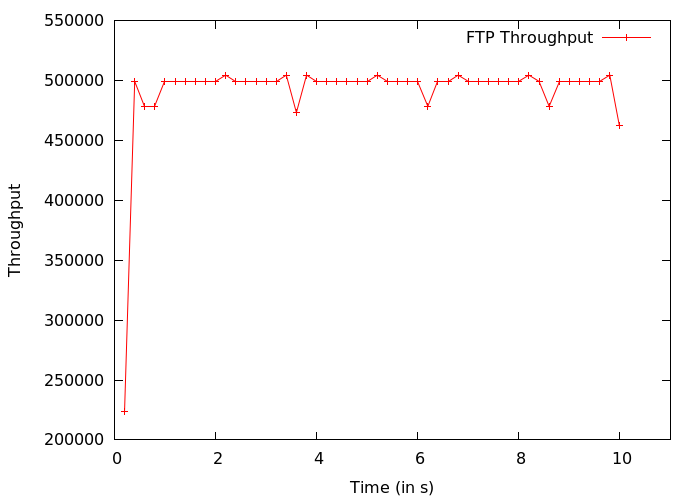
\includegraphics[width = 0.8\linewidth]{./output-ex1-part1-1.png}
 % output-ex1-part1-2-5.png: 700x500 pixel, 72dpi, 24.69x17.64 cm, bb=0 0 700 500
 \caption{Throughput: bandwidth limitation and download connection}
 \label{fig:Q1}
\end{figure}
In figure \ref{fig:Q1} we plotted the throughput of the FTP application. We see that the connection stabilises on 4 Mbps.
The download is limited by the strained connection between node 3 and 4.

\subsection{Question 2}
\begin{figure}[h!]
 \centering
 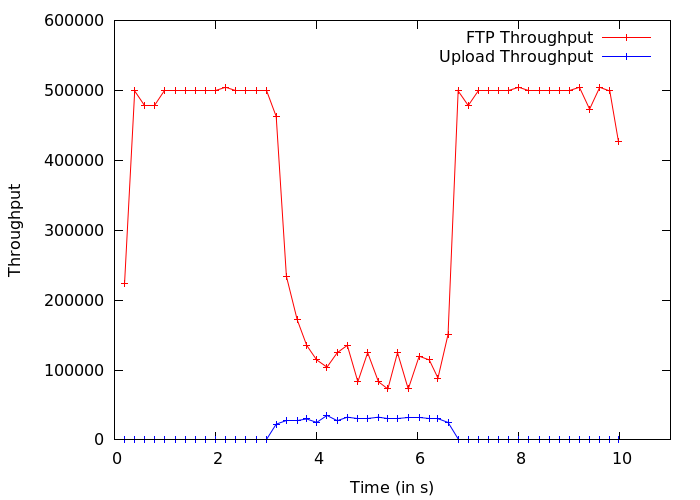
\includegraphics[width = 0.8\linewidth]{./output-ex1-part-2-1-7.png}
 % output-ex1-part-2-1-7.png: 700x500 pixel, 72dpi, 24.69x17.64 cm, bb=0 0 700 500
  \caption{Throughput: bandwidth limitation, download and upload connection}
 \label{fig:Q2}
\end{figure}
The FTP application uses all the available bandwidth. As soon as the CBR pplication starts it clogs up the network. It's packages are bigger than the tcp acknowledgement packages and it takes quite a while to upload them through the constrained upload link. Therefore we see a big drop in the graph, because the delivery of the FTP ACK-packets is delayed. In figure \ref{fig:Q1} we can see a sawtooth behaviour for the FTP throughput in the drop. Between the CBR packets, some ACK's of the FTP appliction get through the strained upload connection.

\subsection{Question 3}
A reserved amount of upload bandwidth for each application would prevent cannibalisation of the connection. A certain throughput would be guaranteed for both applications. Initially the FTP application would behave just like in question 1. When the CBR application starts, it's bandwidth will decrease because the CBR application has it's own guaranteed bandwidth.

\subsection{Question 4}
\begin{figure}[h!]
 \centering
 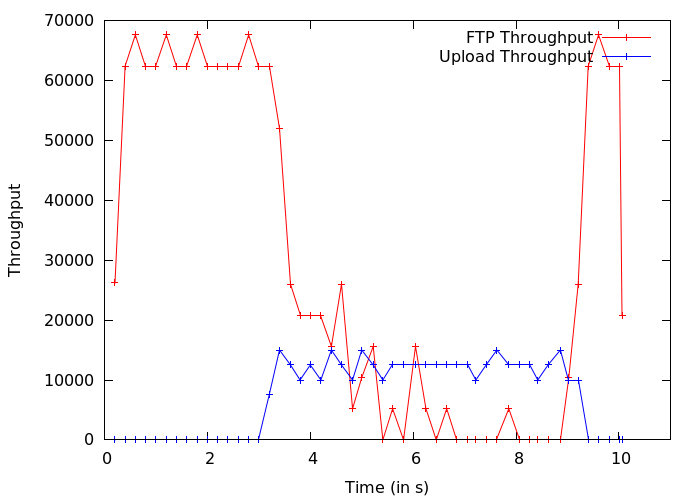
\includegraphics[width = 0.8\linewidth]{./output-ex1-part-4-1-7.png}
 % ex1-part-4-1-7.png: 700x500 pixel, 72dpi, 24.69x17.64 cm, bb=0 0 700 500
 \caption{Throughput: bandwidth limitation, download and upload: even more restricted}
 \label{fig:Q4}
\end{figure}
If the bandwidth is even more constrained, the saturation of the network is even higher as you can see in figure \ref{fig:Q4}. It's worse because it takes longer for the ACK's to arrive. The throughput of the FTP application crashes to zero.

\subsection{Question 5}
\begin{figure}[h!]
 \centering
 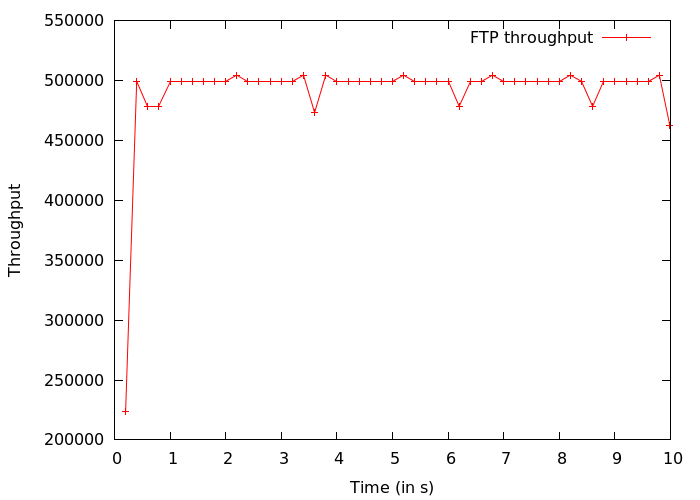
\includegraphics[width = 0.8\linewidth]{./output-ex1-part5.png}
 % output-ex1-part5.png: 700x500 pixel, 72dpi, 24.69x17.64 cm, bb=0 0 700 500
 \caption{Throughput: upload rate at 30 000}
 \label{fig:Q5}
\end{figure}
When the CBR upload connection is fixed to a rate of 30 kbps the FTP connection is not hindered by it as you can see in figure \ref{fig:Q5}.
To prevent hosts from interfering with each other, you could implement some sort of load balancing between hosts. In practice this would result in a (weighted) round-robin queue instead of a FIFO queue.  

\subsection{Question 6}
\subsubsection{Question 6.1}
Since the capacity has a linear increase relative to the load, we see a result similar to question 1
of this exercise. TCP will be responsible for equally distributing the bandwidth amongst the clients. Since big downloaders put more data into the network, they'll have more packets dropped. These big downloaders will then restrict their dataflow.\\ 
In the case where only 5 clients are connected with the modem we see a doubling in bandwidth used by each client. There are fewer connections competing for the same bandwidth.

\subsubsection{Question 6.2}
When the users perform their activities at random times, we expect varying performance. This is because not all the nodes will be active at the same time. In the worst case we get the performance like in the non-random case with 10 users. \\
If some users always send data when the DropTail queue is full, their packets will always be dropped. A different queue design (like round-robin) could aleviate this situation.

\section{Exercise 2}
\subsection{Question 1}
\begin{figure}[h!]
 \centering
 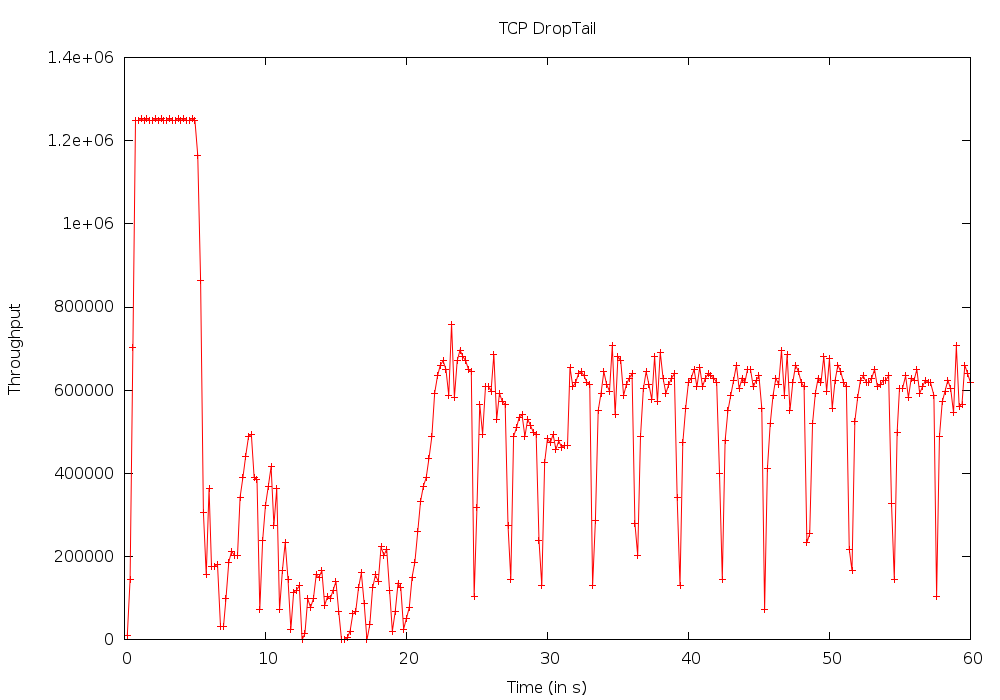
\includegraphics[width = 0.9\linewidth]{./ex2-part1-tp.png}
 \caption{Throughput main FTP connection}
 \label{fig:Q21}
\end{figure}
\begin{figure}[h!]
 \centering
 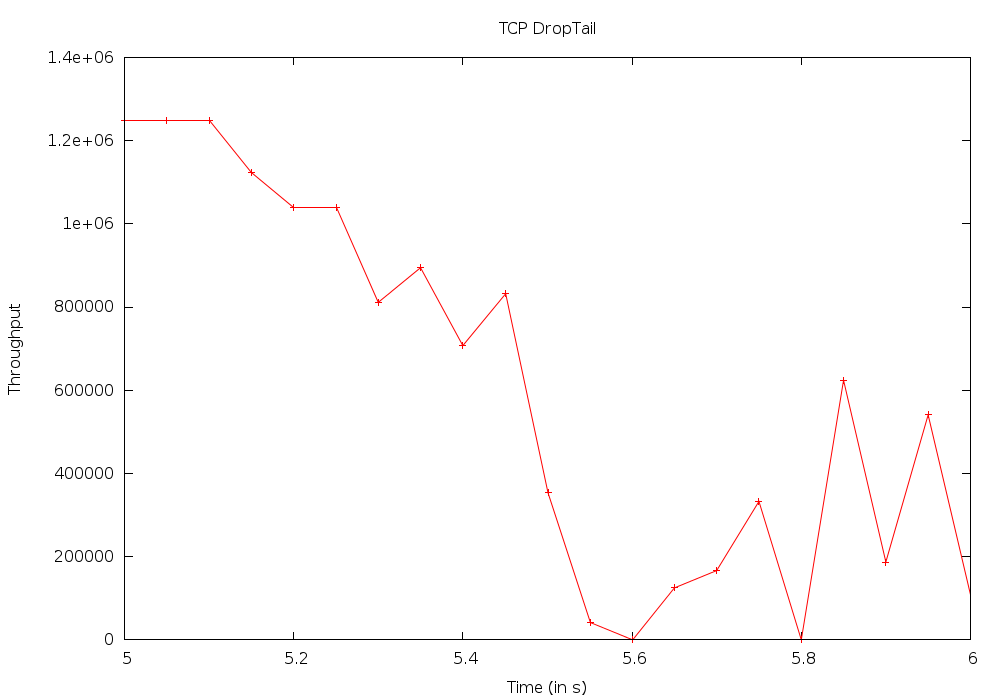
\includegraphics[width = 0.9\linewidth]{./ex2-part1-zoom.png}
 \caption{Throughput main FTP connection (zoomed in)}
 \label{fig:Q211}
\end{figure}

At 5s the throughput of the main FTP application drops, because of the burst connections to the 
webserver. In figure \ref{fig:Q21} and \ref{fig:Q211} we see that the throughput does not drop
immediately at 5s. This is because the different connections to the webserver do not start
immediately at 5s but at randomly from 5s to 7s.

\subsection{Question 2}
\begin{figure}[h!]
 \centering
 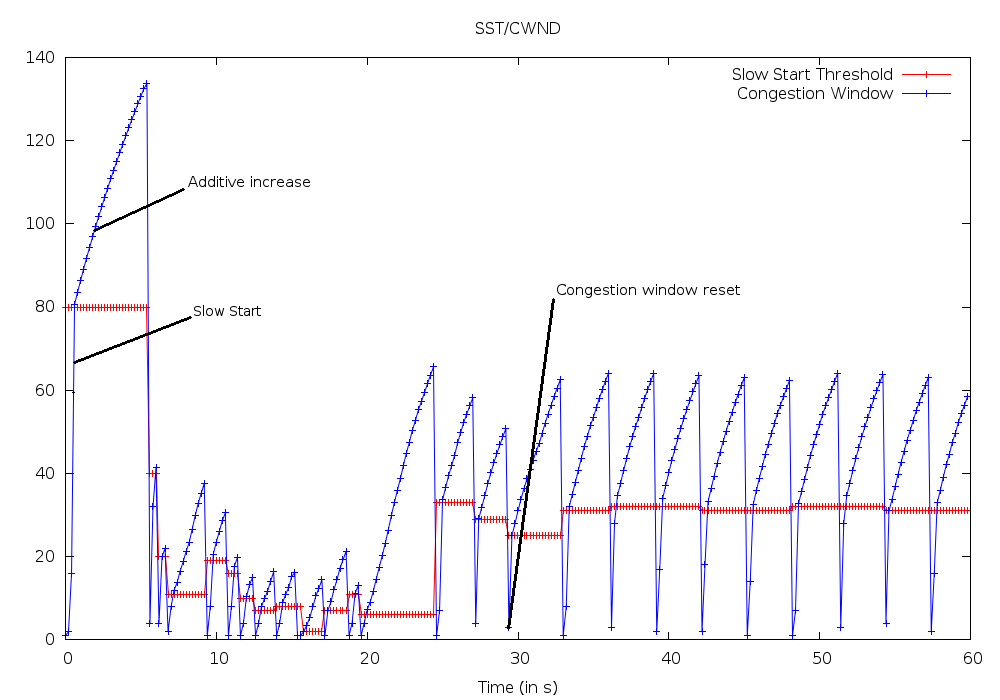
\includegraphics[width = 0.9\linewidth]{./ex2-part1-cwnd-sst.png}
 \caption{Throughput main FTP connection}
 \label{fig:Q22}
\end{figure}
The different phases of the TCP algorithm are annotated on the graph in figure \ref{fig:Q22}.
At first we see the slow start. After we reach the slow start threshold we reach the additive increase phase. When the connection times out/ to many packets are lost, the congestion window is set
to 1 and the slow start threshold is set at half of the reached window size.

\subsection{Question 3}

\subsection{Question 4}

\end{document}
